\section{Definisi \textit{Micro Frameworki}}

\textit{Microframework} adalah istilah yang digunakan untuk merujuk pada kerangka kerja web minimalis. Kerangka ini sangat berbeda dengan kerangka kerja tumpukan penuh. Juga tidak memiliki sebagian besar fungsionalitas secara umum yang ada dalam kerangka kerja aplikasi web lengkap, seperti:
\begin{enumerate}
\item Akun, otentikasi, otorisasi, peran, dll.
\item Abtraksi basis data melalui pemetaan objek-relasional.
\item Validai  \textit{input} dan sanitasi \textit{input}.
\item Mesin \textit{template web}.
\end{enumerate}

Biasanya, sebuah \textit{microframework} memfasilitasi untuk menerima permintaan HTTP, merutekan permintaan HTTP ke \textit{controller} yang sesuai, mengirim \textit{controller}, dan mengembalikan respons HTTP. \textit{Microframeworks} seringkali dirancang khusus untuk membangun API untuk layanan atau aplikasi lain. Misalnya, Lumen \textit{microframework} yang dirancang untuk pengembangan \textit{Microservices} dan pengembangan API. \textit{Microframework} merupakan sebuah \textit{tool} yang digunakan untuk \textit{project} yang lebih kecil dan penggunaan untuk kasus yang spesifik. Ini sama saja dengan menyederhanakan \textit{framework} agar lebih mudah dalam implementasi dan menyediakan \textit{testing} dan \textit{deployment} yang lebih cepat. \textit{Microframework} mengeluarkan banyak sekali komponen yang ada pada pengaturan \textit{full-stack}, termasuk diantaranya:
\begin{enumerate}
\item \textit{Web template engine;}
\item \textit{Input validation;}
\item \textit{Database abstraction;}
\item \textit{Roles, accounts, and authentication.}
\end{enumerate}

Kerugian menggunakan  \textit{microframework} adalah saat  \textit{project} mulai tumbuh besar dengan cepat, dimana  \textit{microframework} tidak memiliki fitur yang dibutuhkan untuk mengakomodasi pertumbuhan  \textit{website}. Dengan kata lain kamu kehilangan fleksibelitas.  \textit{Micro-framework} lebih baik saat digunakan untuk  \textit{project} kecil yang membutuhkan kesederhanaan,  \textit{overhead} yang rendah dan  \textit{deployment} yang cepat.  \textit{Developer} yang sudah berpengalaman bisa saja menggunakan  \textit{microframework} pada awal  \textit{project} dan menambahkan tambahan  \textit{microframework} jika diperlukan. Hal ini merupakan pilihan yang menarik, tetapi untuk pemula dan  \textit{developer} menengah harus menghindari ini \cite{fadhilnet}.

\section{Jenis-Jenis \textit{Framework} Python serta Kelebihan dan Kekurangan}

\subsection{Django}

Django adalah kerangka kerja web Python yang memungkinkan individu dalam pengembangan yang bersih dan cepat. Kerangka kerja web secara umum dikatakan sebagai campuran komponen yang membantu pengembang mengembangkan situs web lebih cepat dan mudah. Karena itu, ini adalah kerangka kerja sumber bebas dan terbuka. Ini dapat disebut sebagai kerangka kerja yang memungkinkan pengembang untuk mengambil konsep penyelesaian secepat mungkin. Django sebagai kerangka kerja membantu mengurangi beberapa kesalahan keamanan umum yang dapat diawasi dengan mudah saat mengembangkan aplikasi. Skalabilitas adalah fitur lain yang disediakan oleh kerangka ini.

Django memiliki \textit{tagline "The web framework for perfectionists with deadlines"}, bagaimana tidak, karena secara \textit{default} Django sudah memiliki berbagai modul umum yang biasa digunakan ketika mengembangkan aplikasi web.

Kelebihan:
\begin{enumerate}
\item Cepat.

Ini telah dirancang sedemikian rupa untuk membantu pengembang membuat aplikasi secepat mungkin. Dari ide, produksi hingga rilis, Django membantu menjadikannya efektif dan efisien. Dengan demikian itu menjadi solusi ideal bagi pengembang yang memiliki fokus utama pada tenggat waktu.

\item Penuh dimuat.

Ini bekerja dengan cara yang mencakup puluhan tambahan untuk membantu dengan otentikasi pengguna, peta situs, administrasi konten, umpan RSS, dan banyak lagi hal-hal seperti itu. Aspek-aspek ini membantu dalam melaksanakan proses pengembangan web sepenuhnya.

\item Aman.

Ketika melakukannya di Django, dipastikan bahwa pengembang tidak melakukan kesalahan yang terkait dengan keamanan. Beberapa kesalahan umum termasuk injeksi SQL, pemalsuan permintaan lintas situs, clickjacking dan skrip lintas situs. Untuk mengelola nama pengguna dan kata sandi secara efektif, sistem otentikasi pengguna adalah kuncinya.

\item Dapat diukur.

Untuk memenuhi permintaan lalu lintas terberat, manfaat kerangka Django dapat dilihat. Oleh karena itu, situs tersibuk menggunakan media ini untuk dengan cepat memenuhi permintaan lalu lintas.

\item Serbaguna.

Manajemen konten,\textit{ platform} komputasi ilmiah, dan bahkan organisasi besar, semua aspek ini dikelola secara efisien dengan penggunaan Django.

\item Dokumentasi yang sangat lengkap dan kamu tidak perlu banyak - banyak \textit{googling} karena sudah disediakan contoh.
\item Modul administrasi yang \textit{auto generate} sesuai dengan model yang didefinisikan di dalam aplikasi. Lebih dari sekedar \textit{CRUD generator}.
\item Sistem migrasi \textit{database} otomatis yang tidak perlu kamu tulis \textit{script}-nya. Cukup mengubah class dan struktur \textit{database} pun berubah sesuai perubahan terakhir.
\item Memiliki sistem form yang kokoh.
\item Sudah \textit{built-in} untuk sistem autentikasi dan roles bila Anda menggunakan \textit{relational database} yang didukung Django seperti MySQL dan PostgreSQL.
\item Memiliki ekstensi - ekstensi yang bisa membuat kamu lebih produktif seperti \textit{Django Rest Framework, Django Rest Auth, Django Celery, Django Mongoengine, GeoDjango,} dan lainnya.
\item Memiliki \textit{template engine} sendiri yang lebih \textit{powerful}.
\item Kompatibilitas dengan berbagai modul dan \textit{library} lain.
\end{enumerate}

Kekurangan:
\begin{enumerate}
\item Menggunakan pola perutean, tentukan URL-nya
\item Django terlalu monolitik
\item Semuanya didasarkan pada Django ORM
\item Komponen dikerahkan bersama
\item Pengetahuan tentang sistem lengkap diperlukan untuk bekerja.
\end{enumerate}

\subsection{Flask}

Python adalah Flask, yang merupakan kerangka kerja mikro untuk Python berdasarkan teknologi seperti Werkzeug, Jinja 2. Flask pada dasarnya adalah kerangka kerja web Python yang dibangun dengan inti kecil dan selanjutnya mudah untuk memperpanjang ekstensi Flask lebih berorientasi Python daripada Django karena beberapa alasan yang jelas. Karena ada sedikit kode \textit{boilerplate} yang harus ditangani oleh pengembang, Flask adalah kerangka kerja web yang mungkin tidak perlu dikerjakan pengembang lebih lama untuk memahami mereka. Banyak aplikasi terkenal di luar sana ditulis dalam kerangka kerja Flask seperti Pinterest, LinkedIn dan halaman web komunitas untuk Flask itu sendiri \cite{ramdani2018clustering}.

Flask sendiri dapat dikatakan sebagai \textit{web framework} yang fleksibel terhadap library apapun untuk Python. Selain itu dokumentasinya yang jelas membuat Flask sangat diminati oleh kawula muda.

Kelebihan:
\begin{enumerate}
	\item \textit{Framework} yang mudah untuk digunakan dan dipahami.
	\item Berisi pengembangan server dan \textit{debugger}.
	\item \textit{RESTfull request dispatching}.
	\item Menggunakan Jinja2 \textit{template engine}.
	\item Dukungan untuk \textit{secure cookies} pada sisi \textit{client}.
	\item 100\% \textit{Web Server Gateway Interface} (WSGI).
	\item Berbasis \textit{Unicode} yaitu suatu standar yang dirancang untuk mengizinkan \textit{text} dan \textit{symbol} dari semua tulisan untuk menampilkan dan dimanipulasi secara konsisten oleh komputer.
	\item Dokumentasi yang ekstensif.
	\item Kompatibilitas \textit{Google App Engine}.
\end{enumerate}

Kekurangan:
\begin{enumerate}
\item Fungsionalitas
\end{enumerate}

Beberapa fitur Flask yang perlu kamu ketahui antara lain:
\begin{enumerate}
	\item \textit{Built-in development server} dan \textit{debugger}.
	\item Terintegrasi dengan unit \textit{testing}.
	\item RESTful.
	\item Menggunakan \textit{template engine} Jinja2.
	\item Mendukung \textit{secure cookie}.
	\item 100\% mendukung WSGI 1.0.
	\item \textit{Unicode based}.
	\item Dokumentasi yang baik.
	\item Komunitas yang kuat.
\end{enumerate}

\subsection{Tornado}

Tornado adalah salah satu kerangka kerja web terbaik dari bahasa pemrograman Python. Kerangka kerja ini memungkinkan pendekatan yang lebih bersih untuk pemrograman server Web dan memiliki fokus yang tajam pada operasi non-pemblokiran, dapat meningkatkan skala ke sejumlah besar koneksi terbuka \cite{panjaitan2018sistem}.

Kelebihan:
\begin{enumerate}
\item Dukungan bawaan

Tornado hadir dengan dukungan bawaan dan menemukan solusi untuk sebagian besar aspek pengembangan Web yang membosankan seperti template, pelokalan, cookie yang ditandatangani, dll. Tornado juga memungkinkan pengguna untuk mencampurnya dengan kerangka kerja lain, dengan cuplikan yang sesuai, sesuai untuk kebutuhan mereka.

\item Koneksi serentak

Tornado menawarkan layanan waktu nyata dan mendukung sejumlah besar koneksi konkuren, streaming HTTP (protokol komunikasi yang diterapkan oleh Apple Inc) dan polling panjang (ini adalah teknologi sembur, yang memungkinkan mekanisme pendorong emulatif dalam keadaan di yang dorongan nyata tidak mungkin). Dengan Tornado, sangat mudah untuk menulis layanan waktu nyata. FriendFeed memelihara koneksi terbuka, terutama untuk penggunanya yang sering terlibat.

\item Kinerja tinggi.

Ini adalah fitur paling menarik dari Tornado. Ini sangat cepat dibandingkan dengan semua kerangka kerja Python Web lainnya. Mempertimbangkan keluaran dasarnya, kecepatannya sekitar empat kali lebih tinggi dan juga cukup efisien.
\end{enumerate}

Tornado memiliki beberapa modul utama seperti:
\begin{enumerate}
\item \textit{Web framework}.
\item \textit{HTTP Server and Client}.
\item \textit{Asynchronous Networking, Coroutines and Concurrency}.
\item \textit{Utilities}.
\end{enumerate}

\subsection{Falcon}

Falcon merupakan pustaka WSGI yang membantu membangun API web dengan kecepatan lebih cepat. Saat Anda membuat kerangka HTTP API selain Falcon dapat memuat banyak dependensi dan abstraksi yang tidak diperlukan. Falcon, di sisi lain, mengurangi semua ketergantungan dan menyediakan pengembang untuk mengembangkan desain yang lebih bersih yang memungkinkan gaya arsitektur HTTP dan REST\cite{azzahra2017karya}.

Falcon mengklaim bahwa ia dapat menangani lebih banyak permintaan dengan perangkat keras yang sama jika sedang ditangani oleh kerangka kerja lain. Kerangka kerja ini bertujuan untuk memiliki cakupan kode 100\%, sehingga membuatnya lebih andal. Sebagian besar fitur di atas dimungkinkan karena Falcon hanya mempertahankan 2 dependensi pihak ketiga seperti enam, mimeparse. Sesuai dengan halaman Falith Github perusahaan seperti RackSpace, OpenStack dan LinkedIn menggunakan Falcon.

Dengan tagline \textit{The Minimalist Python WSGI Framework}, Falcon siap menyuguhkan berbagai fitur yang dapat mempermudah kamu membangun sebuah RESTful API. Falcon merupakan \textit{high performance web framework} yang dapat digunakan untuk membangun HTTP API dan backend apps. %Pengembangan Falcon dimonitori oleh \textit{Rackspace}. 

Kelebihan:
\begin{enumerate}
\item Cepat

Salah satu persyaratan paling penting dari cloud API adalah mereka harus menanggapi permintaan secepat mungkin. Ini menjadi fitur penting dalam skenario real-time ketika jumlah permintaan bersamaan tinggi. Falcon adalah salah satu kerangka kerja tercepat yang tersedia.

\item Cahaya

Kerangka kerja dengan jejak ketergantungan yang lama menjadi sangat sulit untuk disatukan dalam berbagai lingkungan karena pembatasan yang diberlakukan oleh ketergantungan tersebut. Falcon hanya memiliki dua dependensi: enam (pustaka kompatibilitas Python 2 dan 3, yang memfasilitasi basis kode untuk bekerja pada Python 2 dan 3 tanpa memerlukan perubahan apa pun) dan mimeparse (yang menyediakan fungsi seperti parsing nama tipe-mime). Ini membuat Falcon lebih mudah untuk diuji dan digunakan.

\item Fleksibel

Falcon tidak membatasi pengembang ketika memilih perpustakaan sehubungan dengan database, otorisasi, dll. Pengembang dapat memilih perpustakaan yang mereka sukai, yang cocok dengan persyaratan skenario proyek saat ini.
\end{enumerate}

Kekurangan:
\begin{enumerate}
\item Tidak cocok untuk melayani halaman HTML.
\item Belum tentu lebih cepat daripada Flask.
\end{enumerate}

\subsection{Hug}

Hug adalah kerangka kerja berbasis web Python yang lain memberi para pengembang fleksibilitas mengembangkan API dan memungkinkan dapat mengkonsumsinya sesuka mereka. Pengembangan API telah disederhanakan secara drastis melalui beberapa antarmuka. Biarlah itu pengembangan lokal atau melalui HTTP atau bahkan melalui antarmuka baris perintah (CLI), sejauh ini merupakan cara modern tercepat untuk mengembangkan API. Kerangka kerja Hug telah dibangun dengan fokus tunggal pada kinerja dalam pikiran. Dikatakan mengkonsumsi sumber daya hanya bila diperlukan dan selanjutnya dikompilasi menggunakan Cython untuk mencapai angka-angka luar biasa pada kinerja. Dengan semua alasan yang jelas ini, Hug mencuri mahkota sebagai kerangka kerja web tercepat untuk Python 3.

Kelebihan:
\begin{enumerate}
\item Jadikan mengembangkan API yang digerakkan oleh Python sesingkat definisi tertuli.
\item Kerangka kerja harus mendorong kode yang mendokumentasikan sendiri.
\item Itu harus cepat. Pengembang seharusnya tidak pernah merasa perlu mencari di tempat lain karena alasan kinerja.
\item Tes penulisan untuk API yang ditulis di atas pelukan harus mudah dan intuitif.
\item Sihir yang dilakukan sekali, dalam kerangka kerja API, lebih baik daripada mendorong masalah yang disetel ke pengguna kerangka API.
\item Menjadi dasar untuk API Python generasi berikutnya, merangkul teknologi terbaru.
\end{enumerate}

Kekurangan:
\begin{enumerate}
\item Hanya dapat memuat kode sedikit.
\end{enumerate}

\subsection{Sanic}

Sanic adalah kerangka kerja web Python \(cocok untuk Python 3.5\) yang dibangun di atas \textit{uvloop} dan dirancang untuk respons HTTP yang lebih cepat melalui penanganan permintaan yang tidak sinkron. Karena struktur internal dan ketergantungannya yang kuat pada uvloop, itu tidak dapat dikembangkan atau digunakan pada lingkungan Windows. Sampai saat ini, Sanic masih dalam tahap pengembangan dan dianggap sebagai bayi di antara kerangka web lain yang tersedia untuk Python. Dengan ini, ada sejumlah kode yang telah ditulis di sekitar Sanic agar Anda dapat menggunakannya untuk keperluan bisnis yang kompleks. Mengingat masih dalam pengembangan, tidak ada banyak aplikasi atau ekstensi untuk Sanic dibandingkan dengan Flask atau Django. Mengingat semua itu, kerangka kerja ini memungkinkan Anda untuk mengambil keuntungan dari sintaks async atau menunggu untuk mendefinisikan fungsi asinkron Anda sendiri. Ini memberikan kekuatan menulis aplikasi asinkron seperti apa yang dapat dicapai dengan menggunakan Node.js.

Kelebihan:
\begin{enumerate}
\item Server yang dikonfigurasikan untuk harus dilampirkan ke aplikasi yang ada.
\item Aplikasi Sanic dapat menentukan rute reguler yang akan hidup berdampingan dengan server Engine.IO. Pola khas adalah menambahkan rute yang melayani aplikasi klien dan file statis terkait dengan aplikasi ini.
\end{enumerate}

Kekurangan:
\begin{itemize}
\item Tidak memiliki banyak aplikasi atau ekstensi.
\end{itemize}

\subsection{Aiohttp}

Kerangka kerja asinkron yang sangat bergantung pada dan menggunakan fitur Python 3.5+ seperti async dan menunggu. Kerangka kerja ini tidak hanya kerangka kerja server web tetapi juga bertindak sebagai kerangka kerja klien juga, karena mendukung baik WebSocket Server dan Klien. Ini adalah kerangka kerja terkenal yang memanfaatkan perpustakaan asinkron populer - asyncio yang ada di sana sejak awal perpustakaan. aiohttp seperti Flask menyediakan objek permintaan dan router untuk memungkinkan pengalihan permintaan ke fungsi yang dikembangkan untuk menanganinya. Sebagai pengembang layanan-mikro, Anda bisa fokus membangun pandangan seperti yang akan Anda lakukan dengan Flask.

Kelebihan:
\begin{enumerate}
\item Efisiensi.

Menangani jumlah permintaan yang setara dengan server yang lebih sedikit atau lebih kecil dibandingkan dengan sinkronisasi. Skalabilitas dibatasi oleh jumlah koneksi soket terbuka dalam proses tunggal vs. jumlah utas\/proses bersamaan untuk sinkronisasi kerangka kerja web (ribuan hingga puluhan ribu untuk async vs. puluhan hingga ratusan untuk sinkronisasi). Server kecil (dalam hal CPU dan memori) menjalankan web async layanan dalam satu proses akan cocok dan seringkali mengungguli yang lebih besar server menjalankan layanan web sinkronisasi menggunakan puluhan hingga ratusan utas/proses.

\item Mampu menangani sejumlah besar permintaan bersamaan.

Mengizinkan fungsionalitas \textit{push} yang efisien melalui soket web, EventSource, atau koneksi berumur panjang lainnya
\end{enumerate}

Kekurangan:
\begin{itemize}
\item Tunggal.

Memiliki model yang lebih kompleks untuk dipikirkan status bersama dan bagaimana hal itu dapat berubah dari satu proses sinkronisasi, harus diingat bahwa status bersama dapat berubah di antara saat-saat menghasilkan kontrol ke loop acara dan mengembalikan kontrol ke kode Anda.
\end{itemize}

\subsection{Piramid}

Kerangka kerja yang telah dikembangkan atau dibangun untuk aplikasi yang lebih besar. Piramida, nama itu sendiri menunjukkan bahwa itu fleksibel, tidak seperti Django yang menawarkan pendekatan "semuanya di dalam kotak". Aplikasi web dibangun menggunakan Pyramid, mulai dari modul file tunggal dan kemudian proyek-proyek ini berkembang menjadi proyek yang lebih besar dan ambisius dalam waktu singkat. Kerugian dari kerangka kerja web ini adalah dokumentasi mereka sendiri, yang tidak terlalu jelas dan terkadang membingungkan. Chameleon Pyramid dipasang untuk menggunakan templat Chameleon alih-alih templat Jinja. Dibutuhkan beberapa waktu dalam mengembangkan aplikasi file tunggal dengan Pyramid, tetapi kemudian, ini dapat ditingkatkan lebih cepat karena pengaturan awal lebih keras dan rawan kesalahan.

Kelebihan:
\begin{enumerate}
\item Fleksibilitas.

Sistem rendering template, cara menyambungkan ke database, cara memetakan url ke tampilan , semacam sistem otentikasi, dan banyak hal lainnya. Piramida sangat bagus karena semua komponen ini dapat ditukar. Anda dapat memilih mesin rendering template, memiliki dua cara berbeda untuk memetakan url ke tampilan dan dapat menggunakannya keduanya di aplikasi yang sama, dapat menggunakan metode apa pun yang ingin disambungkan ke database (meskipun SQLAlchemy umumnya digunakan), dan bahkan dapat terhubung ke beberapa database dari tipe yang sangat berbeda.

\item Kemudahan AJAX.

Penggunaan dekorator dan tampilan XHR membuatnya sangat mudah untuk mendapatkan permintaan AJAX untuk pergi ke tempat yang Anda inginkan. Menjelaskan XHR, dekorator, atau AJAX jauh di luar cakupan tutorial ini, tetapi saya jamin penjelasannya ada di luar sana.

\item Dukungan SQLAlchemy

SQLAlchemy adalah hal yang sangat kuat, banyak orang yang sangat pintar berpikir itu adalah ORM terbaik di sekitar. Jika Anda memilih Django Anda memilih untuk tidak menggunakan SQLAlchemy. Itu hanya masalah besar jika aplikasi Anda sangat (SQL) database intensif - jika Anda ingin melakukan pertanyaan rumit dengan cara yang waras. Di sisi lain, jika aplikasi Anda sederhana maka SQLAlchemy tidak akan banyak membantu, tetapi tidak ada salahnya untuk memilikinya.
\end{enumerate}

Kekurangan:
\begin{enumerate}
\item Fungsionalitas
\end{enumerate}

Beberapa fitur Pyramid:
\begin{enumerate}
\item Kompatibel dengan berbagai template engine seperti Jinja2, Chameleon, dan Mako.
\item Mempunyai sistem form yang handal.
\item Menggunakan SQL Alchemy untuk teknologi database.
\item Memiliki bootstraper.
\item Function decorator.
\item Asset management.
\item Event dan subcriber
\end{enumerate}

\subsection{Web2py}

Merupakan salah satu \textit{full-stack enterprise framework} yang \textit{free} dan \textit{open source} untuk membangun aplikasi web berbasis \textit{database} yang aman. Web2Py merupakan salah satu \textit{web framework} yang masih ada hingga hari ini. Tidak hanya soal \textit{url routing}, Web2Py pun memiliki \textit{template engine} yang cukup \textit{powerful} untuk membuat halaman web. %Hingga saat ini, \textit{framework} ini dikelola oleh 129 kontributor di Github. 

Beberapa fitur yang dimiliki oleh Web2py antara lain:
\begin{enumerate}
\item Dibuat oleh komunitas terpercaya.
\item Selalu backward compatible.
\item Mudah digunakan.
\item Dapat berjalan di banyak sistem operasi.
\item Dapat berjalan di banyak web server.
\item Dapat "berbicara" ke SQLite3, PostgreSQL, MySQL, MSSQL, FireBird, Oracle, IBM DB2, Informix, Ingres, dan Google App Engine.
\item Aman dari cross site scripting, injection flaws, dan eksekusi file berbahaya.
\item Mengajarkan penggunanya apa arti MVC yang sesungguhnya.
\item Kompatibel dengan berbagai protokol seperti REST, RSS, HTML, REST, XML-RPC, dan lainnya.
\item Dukungan berbagai modul dan library yang sudah disediakan oleh Web2py
\end{enumerate}

\subsection{TurboGears2}

TurboGears2 adalah kerangka web berbasis Python yang didasarkan pada paradigma ObjectDispatch. Ini secara khusus dimaksudkan untuk memungkinkan untuk menulis aplikasi kecil dan ringkas dalam mode Minimal dan aplikasi yang jauh lebih kompleks dalam Mode Stack Penuh. Fitur TurboGears2 adalah ORM dengan dukungan multi-database nyata, dan juga mendukung partisi data horizontal, sistem widget untuk menyederhanakan pengembangan aplikasi AJAX.

Kelebihan:
\begin{enumerate}
\item Dukungan Web Server Gateway Interface (WSGI)
\item Sistem widget yang mempermudah pembuatan aplikasi AJAX
\item Mendukung multi data-exchange format
\item Dapat membuat pluggable application
\item Template engine yang sangat designer friendly
\end{enumerate}

Kekurangan:
\begin{enumerate}
\item Fungsionalitas
\end{enumerate}

\subsection{Cherrypy}

CherryPy yang merupakan kerangka kerja berikutnya dalam daftar, yang digunakan untuk menjadi jalan antara masalah dan programmer. Aplikasi web yang dibangun menggunakan kerangka CherryPy terlihat seperti aplikasi Python lainnya dan berjalan tanpa memberikan pengaturan rumit dan penyesuaian terbaik. Bersamaan dengan itu, ia juga memperluas dukungannya ke berbagai jenis server web seperti Apache, IIS dan banyak lagi. Karena itu, CherryPy mengemasnya bersama server web, sehingga aplikasi dapat digunakan di mana pun Python diinstal. Ini juga memungkinkan Anda untuk memulai beberapa server HTTP sekaligus. Tidak ada paksaan yang diberlakukan oleh CherryPy untuk menggunakan mesin templat tertentu, ORM atau pustaka JavaScript dan karenanya kami sebagai pengembang memiliki pilihan untuk memilih mana yang sesuai dengan kebutuhan kami dengan lebih baik.

Kelebihan:
\begin{enumerate}
\item CherryPy berjalan dengan mudah di lingkungan yang kompatibel dengan WSGI seperti server web Apache dan bahkan dapat dijalankan di server mandiri tanpa gangguan langkah otorisasi dan akses backend.
\item Pengembangan aplikasi web adalah tersedianya pilihan penyesuaian, dengan demikian menarik lebih banyak peminat untuk itu. Dan bit penyesuaian hanya dimungkinkan karena CherryPy menawarkan berbagai macam fitur dan alat untuk memungkinkannya bagi pengembang.
\end{enumerate}

Kekurangan:
\begin{enumerate}
\item Tidak memiliki sistem templating sendiri sehingga harus memilih template yang cocok.
\end{enumerate}

CherryPy memiliki dukungan seperti berikut:
\begin{enumerate}
\item URL routing.
\item Static file management.
\item Managable configuration.
\item Kompatibel dengan WSGI dan HTTP/1.1.
\item Built-in profiling, coverage, dan dukungan testing.
\item Dukungan terhadap session, authentication, static content, dan banyak lagi.
\item Dukungan bawaan untuk caching dan encoding.
\item Sistem konfigurasi yang enak.
\end{enumerate}

\section{Instalasi dan Hello World di Flask}

\subsection{Instalasi Python 2.7.}

Mulai dengan tutorial dalam menginstall Python 2.7. Python ini digunakan untuk code pembaca data dari sinyal gelombang otak yang telah dihasilkan oleh alat EEG yaitu NeuroSky Mindwave. Baiklah langsung kita mulai saja:
\begin{enumerate}
\item Pertama-tama silahkan download software dari python versi 2 di laptop anda. Download python versi 2.7.15 dari situs web resminya di www.python.org. Silahkan sesuaikan dengan kapasitas laptop anda, bisa yang win 32 atau yang win 64. Contoh downloadnya seperti pada gambar \ref{fig:python}.
\begin{figure}[!htbp]
	\centerline{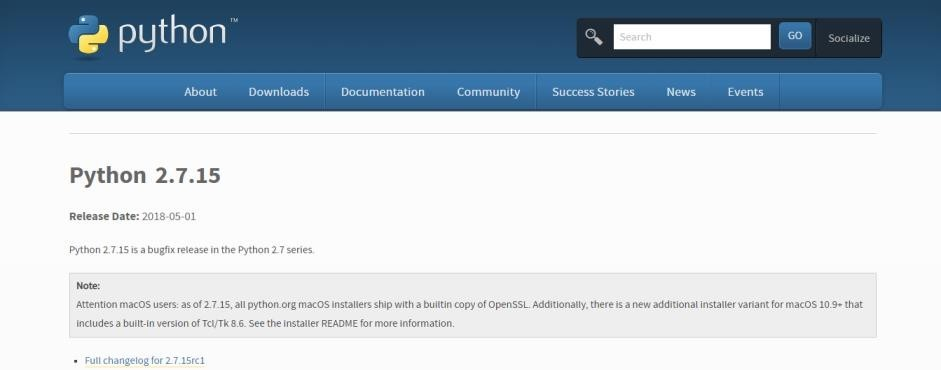
\includegraphics[width=0.85\textwidth]{figures/8/python.jpg}}
	\caption{Download Softfile Python 2.7.}
	\label{fig:python}
\end{figure}

\item Setelah berhasil mendownload mentahan pythonnya silahkan lakukan instalasi seperti biasa anda lakukan. Setelah selesai instalasi pythonnya silahkan cek di \textit{Command Prompt}, apakah python telah terbaca/\textit{running} disesuaikan dengan laptop anda atau belum. Contoh pengecekan di Command Prompt seperti pada gambar \ref{fig:cek_python27}
\begin{figure}[!htbp]
	\centerline{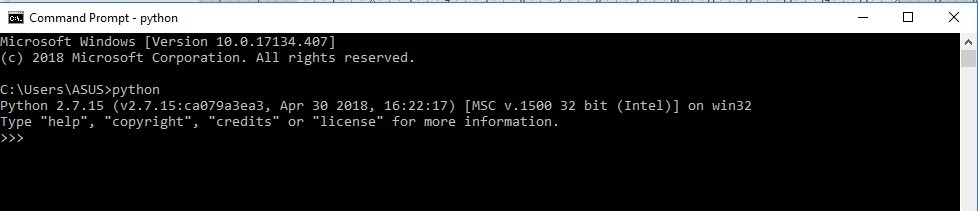
\includegraphics[width=0.85\textwidth]{figures/8/cek_python27.jpg}}
	\caption{Pengecekan Python 2.7.}
	\label{fig:cek_python27}
\end{figure}

\item Apabila tampilannya telah sesuai dengan gambar \ref{fig:cek_python27}, maka python anda siap digunakan.
\item Pastikan python yang terbaca versi 2.7.15 atau bahkan belum ada sama sekali silahkan lakukan konfigurasi ini:
\begin{itemize}
\item Silahkan buka \textit{Control Panel} anda.
\item Pilih System and Security.
\item Kemudian pilih lagi system.
\item Lalu  di  bagian  kiri  tampilan  ada  sub menu  Advanced  system setting.
\item Pada  sub  menu  tersebut  silahkan  pilih  button  Environment Variabel.
\item Silahkan ganti path dengan \verb|C:\Python27| dan \verb|C:\Python27\Scripts| ( Lokasi anda menyimpan mentahan python yang telah anda install tadi ).
\item Maka tampilannya akan seperti pada gambar \ref{fig:editenv}.
\begin{figure}[!htbp]
	\centerline{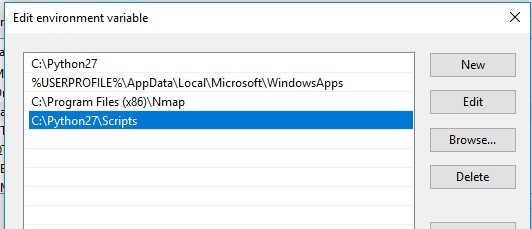
\includegraphics[width=1\textwidth]{figures/8/editenv.jpg}}
	\caption{Pengubahan Environment Python 2.7.}
	\label{fig:editenv}
\end{figure}

\item Jangan lupa untuk memasukkan script dari pythonnya sehingga benar-benar bisa terbaca untuk pipnya. Silahkan klik button ok sampai selesai.
\item Setelah itu, lakukan pengecekan ulang di Command Prompt maka hasilnya akan berubah menjadi versi 2.7.15.
\end{itemize}
\end{enumerate}

\subsection{Instalasi Python 3.6}

Selanjutnya kita mulai dengan tutorial dalam menginstall Python 3.6. Python ini digunakan untuk code pengolahan data csv ke dalam flask python.
\begin{enumerate}
\item Pertama-tama silahkan download software dari python versi 3 di laptop anda. Download python versi 3.6.3 dari situs web resminya yaitu https://www.python.org/. Silahkan sesuaikan dengan kapasitas laptop anda, bisa yang win 32 atau yang win 64 ( 32 bit / 64 bit ). Contoh downloadnya seperti seperti pada gambar \ref{fig:python36}.
\begin{figure}[!htbp]
	\centerline{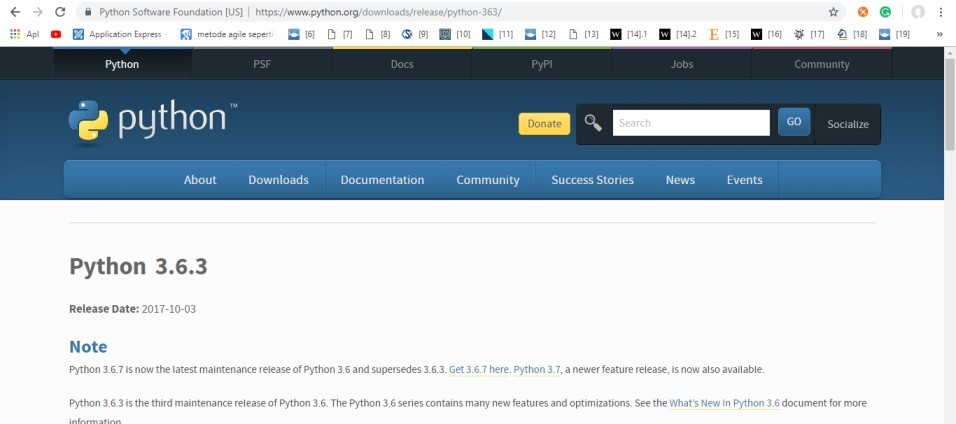
\includegraphics[width=0.85\textwidth]{figures/8/python36.jpg}}
	\caption{Download Softfile Python 3.6.}
	\label{fig:python36}
\end{figure}
 
\item Setelah berhasil mendownload mentahan pythonnya silahkan lakukan instalasi seperti biasa anda lakukan. Setelah selesai instalasi pythonnya silahkan check di Command Prompt, apakah Pythonnya telah terbaca / running disesuaikan dengan laptop anda atau belum. Contoh pengecekan di Command Prompt seperti pada gambar \ref{fig:cek_python36}
\begin{figure}[!htbp]
	\centerline{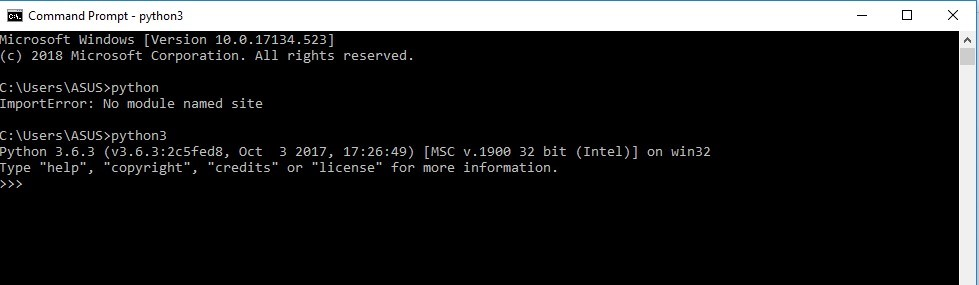
\includegraphics[width=0.85\textwidth]{figures/8/cek_python36.jpg}}
	\caption{Pengecekan Python 3.6.}
	\label{fig:cek_python36}
\end{figure}

\item Apabila tampilannya telah sesuai dengan contoh diatas, maka python anda siap digunakan.
\item Pastikan python yang terbaca versi 3.6.3 atau bahkan belum ada sama sekali silahkan lakukan konfigurasi ini:
\begin{itemize}
\item Silahkan buka Control Panel anda.
\item Pilih System and Security.
\item Kemudian pilih lagi system.
\item Lalu  di  bagian  kiri  tampilan  ada  sub menu  Advanced  system setting.
\item Pada  sub  menu  tersebut  silahkan  pilih  button  Environment Variabel.
\item Silahkan ganti path dengan \verb|C:\Python36| dan \verb|C:\Python36\Scripts| (Lokasi anda menyimpan mentahan python yang telah anda install tadi).
\item Maka tampilannya akan seperti pada gambar \ref{fig:editenv36}.
\begin{figure}[!htbp]
	\centerline{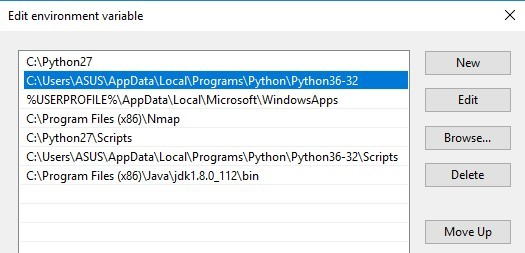
\includegraphics[width=1\textwidth]{figures/8/editenv36.jpg}}
	\caption{Pengubahan Environment Python 3.6.}
	\label{fig:editenv36}
\end{figure}

\item Jangan lupa untuk memasukkan script dari pythonnya sehingga benar-benar bisa terbaca untuk pipnya. Silahkan klik button ok sampai selesai.
\item Setelah itu, lakukan pengecekan ulang di Command Prompt maka hasilnya akan berubah menjadi versi 3.6.3
\item Setelah semua tahap di atas selesai, maka silahkan lanjutkan ke tahap berikutnya.
\end{itemize}
\end{enumerate}

\subsection{Instalasi Framework Flask}
Tutorial selanjutnya ialah kita akan menginstall Framework Flask di komputer/laptop kita sehingga bisa digunakan untuk tutorial selanjutnya. Perlu kita ketahui bahwa flask merupakan \textit{microframework} dari python, dengan penggunaannya, aktivas apapun yang kita lakukan baik pengolahan data dan lain sebagainya akan terasa lebih mudah dan rapih. Ayo kita mulai instalasinya!
\begin{enumerate}
\item Pertama, silahkan nyalakan PC/laptop Anda.
\item Kemudian apabila PC/laptop Anda sudah siap digunakan, silahkan buka web browser seperti Chrome, Mozilla Firefox, dsb.
\item Selanjutnya ketikkan pada web browser Anda alamat laman resmi https://pypi.org/project/Flask/ untuk mengunduh Flask. Contohnya akan nampak seperti pada gambar \ref{fig:download_flask}.
\begin{figure}[!htbp]
	\centerline{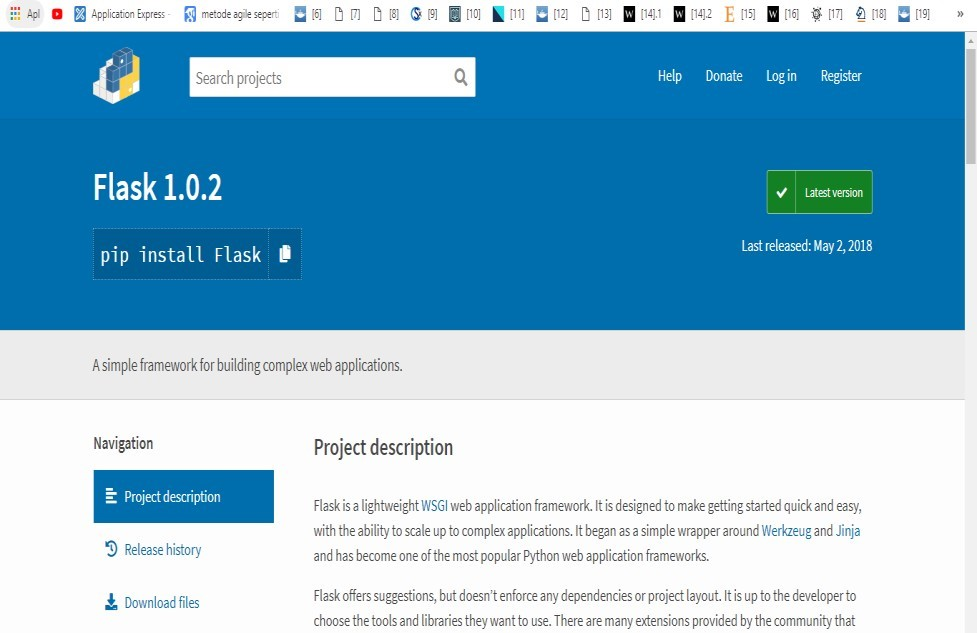
\includegraphics[width=0.85\textwidth]{figures/8/download_flask.jpg}}
	\caption{Download Flask}
	\label{fig:download_flask}
\end{figure}
 
\item Setelah  proses mengunduh selesai, silahkan buka Command Prompt di PC/laptop Anda.
\item Kemudian silahkan ketikkan perintah \verb|pip install flask|.
\item Setelah mengetikkan perintah tersebut, silahkan tekan enter maka prosesnya akan berjalan. Hasilnya akan nampak seperti pada gambar \ref{fig:install_flask}.
\begin{figure}[!htbp]
	\centerline{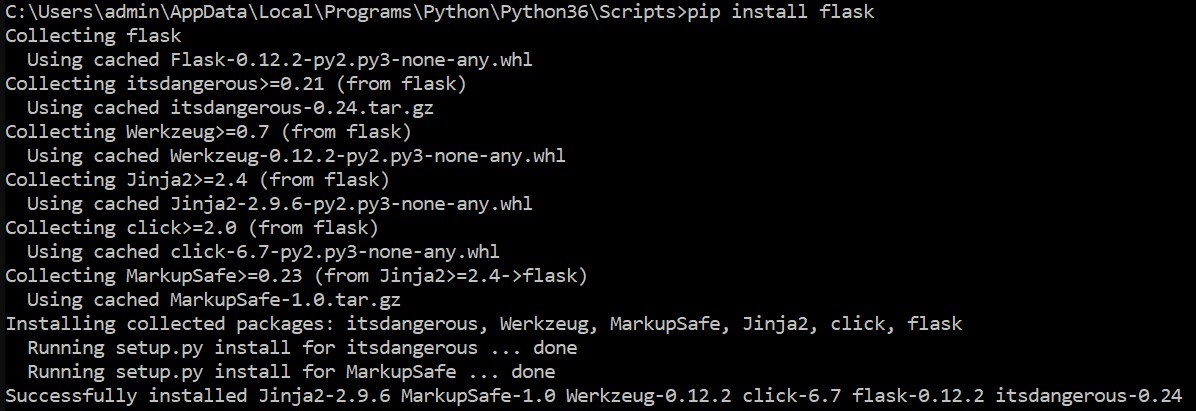
\includegraphics[width=0.85\textwidth]{figures/8/install_flask.jpg}}
	\caption{Proses Instalasi Flask}
	\label{fig:install_flask}
\end{figure}
 
\item Proses intalasi sudah berhasil apabila tampilan pada PC/laptop Anda sudah sama seperti pada gambar \ref{fig:install_flask}. Namun jika masih terjadi \textit{error}, coba lakukan kembali langkah-langkah instalasi flask, dan pastikan Anda telah melakukan semua proses sesuai dengan tutorial di buku ini. Setelah flask sudah terpasang pada PC/laptop Anda, silahkan untuk melanjutkan ke tutorial selanjutnya.
\end{enumerate}

\subsection{Instalasi Library Pandas}

Perlu kita ketahui bahwa pandas merupakan \textit{library} dari bahasa pemrograman python. Library ini digunakan untuk pemrosesan data analitik. Mengapa kita gunakan? Karena memang pandas ini akan mengolah data analitik dari CSV file yang berisikan data sinyal gelombang otak yang bisa kita baca dan tangkap dari aktifitas tertentu (lampu sein saat bermotor). Ayo kita mulai instalasinya!
\begin{enumerate}
\item Pertama silahkan nyalakan PC/laptop Anda.
\item Kemudian apabila PC/laptop Anda sudah siap digunakan, silahkan buka web browser seperti Chrome, Mozilla Firefox, dsb.
\item Selanjutnya ketikkan pada web browser Anda alamat laman resmi https://pypi.org/project/pandas/untuk mengunduh pandas. Contohnya nampak seperti pada gambar \ref{fig:download_pandas}.
\begin{figure}[!htbp]
	\centerline{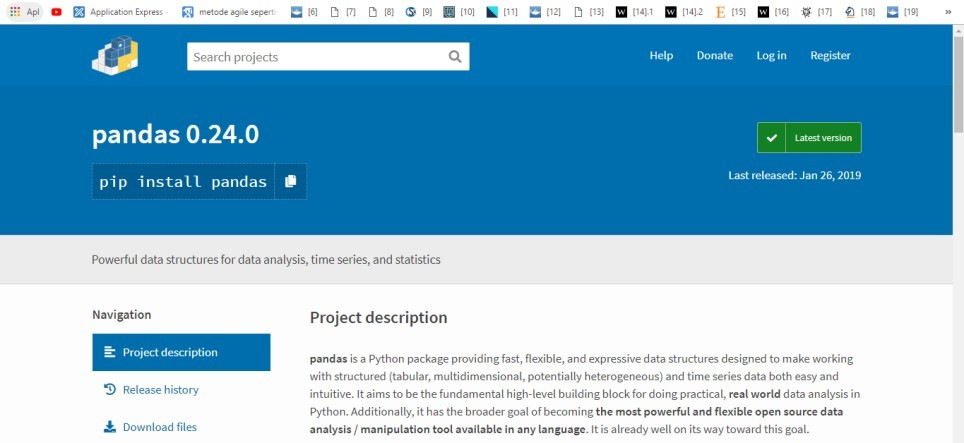
\includegraphics[width=0.85\textwidth]{figures/8/download_pandas.jpg}}
	\caption{Download Pandas}
	\label{fig:download_pandas}
\end{figure}
 
\item Setelah proses mengunduh selesai, silahkan buka Command Prompt di PC/laptop Anda.
\item Kemudian silahkan ketikkan perintah \verb|pip install pandas|.
\item Setelah  mengetikkan  perintah  tersebut,  silahkan  tekan  enter  maka prosesnya akan berjalan. Silahkan tunggu untuk melihat hasilnya yang akan nampak seperti pada gambar \ref{fig:install_pandas}.
\begin{figure}[!htbp]
	\centerline{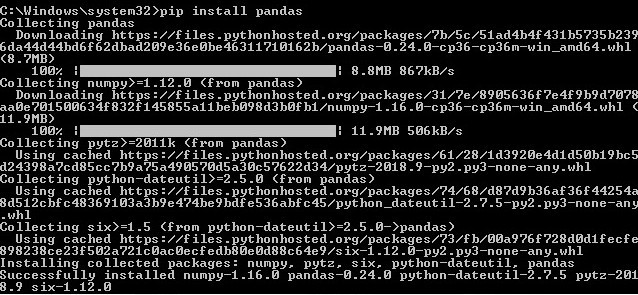
\includegraphics[width=0.85\textwidth]{figures/8/install_pandas.jpg}}
	\caption{Proses Instalasi Pandas}
	\label{fig:install_pandas}
\end{figure}
 
\item  Proses intalasi sudah berhasil apabila tampilan pada PC/laptop Anda sudah sama seperti pada gambar \ref{fig:intsall_pandas}. Namun jika masih terjadi \textit{error}, coba lakukan kembali langkah-langkah instalasi pandas, dan pastikan Anda telah  melakukan semua proses sesuai dengan tutoral di buku ini.
\item Setelah pandasnya terpasang di komputer/laptop anda maka silahkan lanjutkan ke tutorial selanjutnya.
\end{enumerate}

\subsection{Contoh Penerapan Fungsi Pada Flask Python}

Flask adalah kerangka kerja aplikasi web mikro yang ditulis dalam bahasa pemrograman Python dan berdasarkan Werkzeug toolkit dan template engine Jinja2. Berlisensi BSD.

Langkah-langkah membangun Flask:
\begin{enumerate}
\item Pertama, pastikan bahwa python telah terinstal pada komputer.
\item Kemudian install framework python yaitu Flask pada CMD.
\item Buka CMD.
\item Kemudian ketikkan \verb|pip install flask|. Contohnya seperti pada gambar \ref{fig:install_pip}.
\begin{figure}[!htbp]
	\centerline{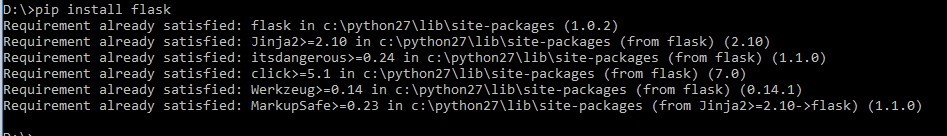
\includegraphics[width=0.85\textwidth]{figures/8/install_pip.jpg}}
	\caption{Instalasi Pip Flask}
	\label{fig:install_pip}
\end{figure} 

\item Gambar   diatas   menunjukkan   bahwa   laptop   anda   telah memiliki flask jadi sudah bisa digunakan.
\item Kemudian masuklah pada \textit{text editor} seperti sublime, $notepad^{++}$, dan lain sebagainya.
\item Kemudian silahkan untuk mulai memasukkan perintah-perintah di Flask.
\item Sebelum mencobanya, alangkah baiknya jika kita mempelajari flask terlebih dahulu.
\item Selanjutnya kita masuk ke bagian perintah python flask. Pada bagian ini kita akan mencoba membuat hello world, berikut ini \textit{source code} untuk membuat hello world seperti pada listing \ref{lst:hello}.
\lstinputlisting[caption=Contoh kode program hello.py, label={lst:hello}]{src/8/hello.py}

 Contoh \textit{source code} main.py bisa dilihat seperti pada listing \ref{lst:main}.
\lstinputlisting[caption=Contoh kode program main.py, label={lst:main}]{src/8/main.py}

\item Masukkan perintah \verb|import hello| untuk memanggil dan menghubungkan fungsi ke dalam file flask ini.
\item Pada file flask juga didefinisikan pemanggilan untuk fungsi hello world nya.
\item Pemanggilannya berupa, apabila parameter word difungsikan maka akan langsung terhubung dengan fungsi hello world dan tulisan hello worldnya akan tampil sesuai dengan request GetSilahkan jalankan file pada CMD, maka hasilnya akan nampak seperti gambar \ref{fig:call_function1}.
\begin{figure}[!htbp]
	\centerline{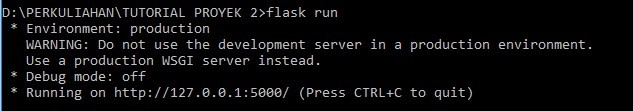
\includegraphics[width=0.85\textwidth]{figures/8/call_function1.jpg}}
	\caption{Pemanggilan Fungsi Flask Opsi 1}
	\label{fig:call_function1}
\end{figure} 
 
\item Atau bisa juga seperti pada gambar \ref{fig:call_function2}.
\begin{figure}[!htbp]
	\centerline{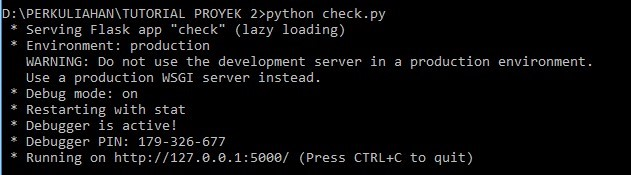
\includegraphics[width=0.85\textwidth]{figures/8/call_function2.jpg}}
	\caption{Pemanggilan Fungsi Flask Opsi 2}
	\label{fig:call_function2}
\end{figure} 
 
\item Copy URL yang ada pada CMD, lalu cek URL di Web Browser. Maka hasilnya akan nampak seperti pada gambar \ref{fig:hello_world}.
\begin{figure}[!htbp]
	\centerline{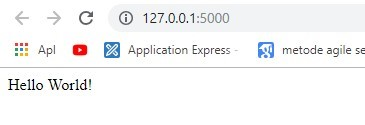
\includegraphics[width=1\textwidth]{figures/8/hello_world.jpg}}
	\caption{Output Hello World}
	\label{fig:hello_world}
\end{figure} 
\end{enumerate} 

\section{Penanganan Error}

\subsection{Penanganan Error pada Python}

Contoh kasus 1: Untuk tutorial ini, akan dicontohkan penanganan error untuk contoh Python. Ini contoh yang pertama. Sebelum menangani error. Akan dijelaskan terlebih dahulu tutorial untuk pembangunan Pythonnya kemudian akan masuk kepada penanganan error yang ada. Silahkan simak dan ikuti tutorial berikut:
\begin{enumerate}
\item Pertama, pastikan bahwa python telah terinstal di PC/laptop Anda. Anda dapat menggunakan python versi 2 maupun python versi 3. Untuk tutorial pertama ini, kita akan menggunakan Python 3.
\item Selanjutnya silahkan buka text editor. Untuk text editornya bisa apa saja. Namun, untuk tutorial ini dicontohkan dengan menggunakan Sublime 3.
\item Selanjutnya silahkan buat script Pythonnya, dengan nama file satu.py. Scriptnya dicontohkan seperti pada tabel dibawah ini:
%Tabel 1. File satu.py
%def hello(nama):
%	sambutan = "Assalamualaikum"
%	penggabungan = sambutan + " " + nama
\item Apabila telah membuat script seperti diatas maka silahkan buka CMD. CMD adalah Command Prompt, software bawaan laptop anda
\item Kemudian pada CMD silahkan masuk ke tempat file anda tersimpan
\item Setelah masuk, silahkan check terlebih dahulu dengan perintah “Python2 1.py “
\item Apabila jalan maka berhasil. Silahkan keluar dari tempat file tersebut. Pada CMD silahkan ketikkan Python3
\item Kemudian silahkan eksekusi fungsi yang ada pada file tersebut untuk melihat hasilnya. Untuk pengeksekusiannya seperti pada gambar dibawah 
%Gambar 1. Eksekusi Fungsi
\item Ketika dieksekusi seperti ini. Tapi kenapa tidak ada hasilnya? Padahal untuk fungsi dan parameternya telah disetting. Coba perhatikan lagi pada script Pythonnya. Ternyata ada yang kurang, selain inputan seharusnya ada keluaran
\item Nah untuk perintah keluarannya belum ada. Untuk perintahnya bisa Print. Silahkan ganti script satu.py seperti contoh berikut:
%Tabel 2. File satu.py
%def hello(nama):
%	sambutan = "Assalamualaikum"
%	penggabungan = sambutan + " " + nama
%	print penggabungan
\item Setelah mengganti script diatas, maka silahkan buka CMD. Masuk ke tempat penyimpanan file.
\item Kemudian ketikan perintah Python3 ( untuk masuk ke Pythonnya )
\item Silahkan eksekusi ulang dengan cara yang sama
\item Hasilnya sebagai berikut:
%Gambar 2. Eksekusi Fungsi
\item Ternyata malah menghasilkan error yang berbeda. Nah untuk error berikut dinyatakan bahwa ada yang salah dengan perintah keluaran diatas.
\item Setelah ditelusuri ternyata salahnya pada penulisan perintah. Mengapa? Dikarenakan kita menggunakan script Python yang sangat sensitif jadi kita harus menyamakan perintah dengan versi Python yang digunakan. Ternyata untuk pemanggilannya tadi kita menggunakan jenis tulisan perintah untuk Python 2. Seharusnya untuk Python3 kita harus menambahkan beberapa tanda yaitu ( ) tanda kurung pada parameternya sehingga bisa dijalankan
\item Silahkan ganti code seperti contoh berikut:
%def hello(nama):
%	sambutan = "Assalamualaikum"
%	penggabungan = sambutan + " " + nama
%	print (penggabungan)
\item Setelah mengganti code seperti contoh diatas maka silahkan buka kembali CMD. Command Prompt lalu masuk ke file tempat penyimpanan file satu.py
\item Silahkan lakukan kembali perintah pemanggilannya sebagai berikut :
%Gambar 3. Eksekusi Fungsi
\item Hasil yang benar akan nampak seperti gambar tersebut. Dimana ketika telah berhasil melakukan penyettingan pada parameter yang dieksekusi maka fungsi dari file tersebut akan mengeluarkan keluaran yang sesuai
\item Keluarannya tentunya akan berupa string. Semuanya sesuai dengan settingan yang telah dibuat pada file satu.py
\end{enumerate}

Contoh kasus 2 : Untuk tutorial ini, akan dicontohkan penanganan error untuk contoh Python. Ini contoh yang kedua. Sebelum menangani error. Akan dijelaskan terlebih dahulu tutorial untuk pembangunan Pythonnya kemudian akan masuk kepada penanganan error yang ada. Silahkan simak dan ikuti tutorial berikut: 
(Contoh kedua ini akan muncul error yang sama namun dengan penyelesaiian yang berbeda dari contoh sebelumnya)
\begin{enumerate}
\item Pertama-tama silahkan pastikan bahwa di laptop anda telah terinstall Python. Python yang digunakan ada Python 2 dan Python 3. Untuk tutorial pertama ini, kita akan menggunakan Python 3.
\item Selanjutnya silahkan buka text editor. Untuk text editornya bisa apa saja. Namun, untuk tutorial ini dicontohkan dengan menggunakan Sublime 3.
\item Selanjutnya silahkan buat script Pythonnya, dengan nama file satu.py. Scriptnya dicontohkan seperti pada tabel dibawah :
def hello(nama):
%	sambutan = "Assalamualaikum"
%	penggabungan = sambutan + " " + nama
\item Apabila telah membuat script seperti diatas maka silahkan buka CMD. CMD adalah Command Prompt, software bawaan laptop anda. Kemudian pada CMD silahkan masuk ke tempat file anda tersimpan. Setelah masuk, silahkan check terlebih dahulu dengan perintah “ Python2 1.py “
\item Apabila jalan maka berhasil. Silahkan keluar dari tempat file tersebut. Pada CMD silahkan ketikkan Python3
\item Kemudian silahkan eksekusi fungsi yang ada pada file tersebut untuk melihat hasilnya. Untuk pengeksekusiannya seperti pada gambar
\item Ketika dieksekusi seperti ini. Tapi kenapa tidak ada hasilnya? Padahal untuk fungsi dan parameternya telah disetting
\item Coba perhatikan lagi pada script Pythonnya. Ternyata ada yang kurang, selain inputan seharusnya ada keluaran. Nah untuk perintah keluarannya belum ada. Untuk perintahnya bisa Return. Contoh yang pertama menggunakan print dan ternyata seharusnya kita menggunakan perintah Return karena lebih sering dan memang seharusnya dipakai untuk pengembalian keluaran pada fungsi Python
\item Silahkan ganti script satu.py seperti contoh berikut:
%def hello(nama):
%	sambutan = "Assalamualaikum"
%	penggabungan = sambutan + " " + nama
%	return penggabungan
\item Setelah mengganti script diatas, maka silahkan buka CMD. Masuk ke tempat penyimpanan file. Kemudian kettikan perintah Python3 ( untuk masuk ke Pythonnya ). Silahkan eksekusi ulang dengan cara yang sama
\item Hasilnya sebagai berikut 
\item Hasil yang benar akan nampak seperti gambar tersebut.
\item Dimana ketika telah berhasil melakukan penyettingan pada parameter yang dieksekusi maka fungsi dari file tersebut akan mengeluarkan keluaran yang sesuai. Keluarannya tentunya akan berupa string
\item Semuanya sesuai dengan settingan yang telah dibuat pada file satu.py
\end{enumerate}

Contoh kasus 3: Untuk tutorial ini, akan dicontohkan penanganan error untuk contoh Python. Ini contoh yang ketiga. Sebelum menangani error. Akan dijelaskan terlebih dahulu tutorial untuk pembangunan Pythonnya kemudian akan masuk kepada penanganan error yang ada. Silahkan simak dan ikuti tutorial berikut: 
\begin{enumerate}
\item Pertama-tama silahkan pastikan bahwa di laptop anda telah terinstall Python. Python yang digunakan ada Python 2 dan Python 3. Untuk tutorial pertama ini, kita akan menggunakan Python 3.
\item Selanjutnya silahkan buka text editor. Untuk text editornya bisa apa saja. Namun, untuk tutorial ini dicontohkan dengan menggunakan Sublime 3
\item Selanjutnya silahkan buat script Pythonnya, dengan nama file dua.py
\item Scriptnya dicontohkan seperti pada tabel dibawah :
%def hello(nama):
%sambutan = "Assalamualaikum"
%penggabungan = sambutan + " " + nama
%return (penggabungan)
\item Apabila telah membuat script seperti diatas maka silahkan buka CMD. CMD adalah Command Prompt, software bawaan laptop anda. Kemudian pada CMD silahkan masuk ke tempat file anda tersimpan. Setelah masuk, silahkan check terlebih dahulu dengan perintah “ Python2 dua.py “
%\item Apabila jalan maka berhasil, silahkan keluar dari tempat file tersebut. Pada CMD silahkan ketikkan Python3, Kemudian silahkan eksekusi fungsi yang ada pada file tersebut untuk melihat hasilnya 
\item Untuk pengeksekusiannya seperti pada gambar dibawah:
\item Ketika dieksekusi, hasilnya nampak seperti gambar diatas.
\item Tapi kenapa tidak ada hasilnya? Padahal untuk fungsi dan parameternya telah disetting. Coba perhatikan lagi pada script Pythonnya. Ternyata ada yang kurang, selain inputan seharusnya ada keluaran. Nah untuk errornya sendiri ternyata ada pada blokingannya. Dimana Python sangatlah sensitif maka scriptnya juga harus benar. Kita harus menyamakan perintah dengan benar. Penangannan errornya yaitu memberikan SPASI ataupun TAB pada perintah untuk memasukkan inputan dengan benar. Harus sesuai dengan perintah yang lainnya agar dapat dieksekusi dengan benar
\item Silahkan ganti script dua.py seperti contoh berikut:
\begin{verbatim}
def hello(nama):
	sambutan = "Assalamualaikum"
	penggabungan = sambutan + " " + nama
	return penggabungan
\end{verbatim}
\item Setelah mengganti script diatas, maka silahkan buka CMD. Masuk ke tempat penyimpanan file. Kemudian kettikan perintah Python3 ( untuk masuk ke Pythonnya ). Silahkan eksekusi ulang dengan cara yang sama
\item Hasilnya sebagai berikut
\item Hasil yang benar akan nampak seperti gambar tersebut.
\item Dimana ketika telah berhasil melakukan penyettingan pada parameter yang dieksekusi maka fungsi dari file tersebut akan mengeluarkan keluaran yang sesuai. Keluarannya tentunya akan berupa string. Semuanya sesuai dengan settingan yang telah dibuat pada file dua.py
\end{enumerate}

Contoh kasus 4: Untuk tutorial ini, akan dicontohkan penanganan error untuk contoh Python. Ini contoh yang empat. Sebelum menangani error. Akan dijelaskan terlebih dahulu tutorial untuk pembangunan Pythonnya kemudian akan masuk kepada penanganan error yang ada. Silahkan simak dan ikuti tutorial berikut: 
\begin{enumerate}
\item Pertama-tama silahkan pastikan bahwa di laptop anda telah terinstall Python. Python yang digunakan ada Python 2 dan Python 3. Untuk tutorial pertama ini, kita akan menggunakan Python 3.
\item Selanjutnya silahkan buka text editor. Untuk text editornya bisa apa saja. Namun, untuk tutorial ini dicontohkan dengan menggunakan Sublime 3. Selanjutnya silahkan buat script Pythonnya, dengan nama file dua.py
\item Scriptnya dicontohkan seperti pada tabel dibawah:
\begin{verbatim}
def hello(nama):
	sambutan = "Assalamualaikum"
	penggabungan = sambutan + " " + nama
return penggabungan
\end{verbatim}
\item Setelah membuat script diatas, maka silahkan buka CMD. Masuk ke tempat penyimpanan file. Kemudian kettikan perintah Python3 ( untuk masuk ke Pythonnya )
\item Silahkan eksekusi mengikuti perintah berikut:
\item Hasil yang benar akan nampak seperti gambar tersebut.
\item Terjadi error pada eksekusi tersebut. Ternyata untuk error ini terjadi karena salah perintah dalam pengeksekusian. Pada perintah tersebut, kita memasukkan “ import dua “. Maka akan masuk ke file dua.py
\item Namun, setelah itu, kita malah memasukkan perintah “ satu.hello(“annisa”). Yang kalau diartikan, maka perintah tersebut ditujukan untuk file satu.py. Maka dari itu, kita harus mengganti perintah yang kita masukkan dalam pengeksekusian. Kalau mengeksekusi file dua.py maka import dan arahan perintahnya harus ke file dua.py
\item Silahkan eksekusi lagi dengan perintah berikut:
\item Apabila perintah telah sesuai, maka akan menampilkan hasil yang seperti contoh diatas. Keluarannya tentunya akan berupa string. Semuanya sesuai dengan settingan yang telah dibuat pada file dua.py. Dengan permasalahan yang sama, apabila kita secara tidak sengaja menemukan error juga ketika mengeksekusi file satu.py maka penyelesaiannya mirip seperti contoh diatas
\item Dimisalkan untuk file satu.py errornya seperti ini:
\item Nah, tentunya kita sudah tau bahwa salahnya pada pemanggilan yang harusnya mengarah kepada file satu.py. Silahkan dibenarkan lagi.
\item Ikuti contoh eksekusi ini untuk mendapatkan hasil yang benar:
\item Nah, penyelesainnya seperti diatas. Kita harus memperhatikan perintah yang kita gunakan untuk eksekusi.
\end{enumerate}

Contoh kasus 5: Untuk tutorial ini, akan dicontohkan penanganan error untuk contoh Python. Ini contoh yang kelima. Sebelum menangani error. Akan dijelaskan terlebih dahulu tutorial untuk pembangunan Pythonnya kemudian akan masuk kepada penanganan error yang ada. Silahkan simak dan ikuti tutorial berikut: 
(Contoh Python ini digunakan dalam pembuatan script python untuk pembacaan gelombang otak)
\begin{enumerate}
\item Pertama-tama silahkan pastikan bahwa di laptop anda telah terinstall Python. Python yang digunakan ada Python 2 dan Python 3. Untuk tutorial pertama ini, kita akan menggunakan Python 2.
\item Selanjutnya silahkan buka text editor. Untuk text editornya bisa apa saja. Namun, untuk tutorial ini dicontohkan dengan menggunakan Sublime 3.
\item Selanjutnya silahkan buat script Pythonnya, dengan nama file coba.py
\item Scriptnya dicontohkan seperti pada tabel dibawah:
\begin{verbatim}
import mindwave, time
import keyboard
import csv

headset = mindwave.Headset('COM4', '1425')
time.sleep(2)
a=0
headset.connect()
print "Connecting..."

while headset.status != 'connected':
    time.sleep(0.5)
    if headset.status == 'standby':
        headset.connect()
        print "Retrying connect..."
print "Connected."

while True:
    print "raw_value: %s : %s" % (headset.raw_value, a)
    writer.writerow({'RawValue': headset.raw_value, 'sign': a})
\end{verbatim}
\item Pada code diatas mendefinisikan perintah dimana fungsinya akan dipanggil dan berhubungan dengan mindwave.py. Seperti contoh perintah headset.connect dimana fungsinya akan diproses di mindwave.py sehingga apabila hasilnya benar dan sesuai maka akan muncul kata “connecting” seperti perintah print diatas. Apabila alat dan code sesuai maka fungsinya akan jalan, baik itu connected, standby dll. 
\item Nah untuk pembacaan sinyalnya, kita menggunakan variabel dari mindwave.py. Untuk variabelnya bisa dicoba yang attention / blink / meditation dll secara bersamaan juga bisa asal perintahnya benar.
\item Perhatikan code ini:
\begin{verbatim}
headset = mindwave.Headset('COM4', '1425')
time.sleep(2)
\end{verbatim}
\item Untuk mengkoneksikan code dengan alat sehingga terhubung maka serial dari alat tersebut harus benar. Portnya yaitu COM4 dapat dilihat dengan cara :
\begin{itemize}
\item Buka pengaturan laptop anda
\item Kemudian pilih device manager
\item Lalu pilih alat yang anda gunakan misalnya : Mindwave Neurosky
\item Apabila telah diklik maka akan muncul portnya yaitu COM4 
\item Untuk serialnya dapat dilihat dari alatnya sendiri 
\item Pengecekannya yaitu di dalam tempat baterai. Serialnya 1425
\item Port dan serial itu beda-beda tergantung dari alatnya masing-masing
\end{itemize}
\item Time.sleep itu gunanya untuk memberikan jeda pembacaan sinyal sehingga nilai gelombang yang dibaca tidak terlalu cepat dan dapat lebih terpantau. Lebih jelasnya lagi, mengapa time.sleepnya bernilai ( 0.001953125 ) dikarenakan :
\item Silahkan perhatikan ini:
\begin{verbatim}
print "raw_value: %s" % (headset.raw_value)
 time.sleep(0.001953125)
\end{verbatim} 
\item Sampling rate dari alat yang digunakan ialah 512Hz jadi tentunya kita harus mengikuti dan menyesuaikannya dengan baik, untuk code dan alatnya. Nah kemudian 512Hz tersebut kita bagi dengan 1 ( detik ) jadi hasilnya akan menjadi jeda antara sinyal yang telah ditangkap/ dibaca dari alat. 1/512 = 0.001953125 . nah nilai itu yang akan menjadi jeda pada code.
 Selain itu. Kita juga harus memastikan apakah benar bahwa dalam 1 detik itu ada 512 data yang dibaca dan ditangkah oleh alat Dan sesuai hasil dari penguijannya sudah dibuktikan dalam setiap detiknya ada sekitar 480-520an data perdetik.
\item Setelah semua langkah di atas telah dilakukan, kita akan mencoba running coba.py melalui cmd, dengan cara :
\item Buka Command Prompt di komputer/laptop anda masing-masing. Silahkan pada CMD arahkan ke folder / directory tempat file coba.py anda simpan
\item Namun sebelum itu pastikan alat sudah terpasang baterai dan lampu indikator berwarna merah. Masukkan USB ke port yang ada di laptop anda. USBnya tentu milik dari alat mindwavenya
\item Kemudian silahkan masukkan perintah python coba.py
\item Apabila pas anda jika terjadi ERROR seperti gambar dibawah ini  
\item ERROR diatas sebenarnya menunjukan bahwa indentasi codingan anda tak sesuai maka yang perlu dilakukan ialah rapikan code anda sesuai dengan perintah-perintah terkait. Biasanya ERROR ini terjadi ketika code anda tak berada pada tempatnya maka silahkan sesuaikan dengan SPACI ataupun TAB. 
\item Silahkan Run kembali
\item Ketika di Run, dan terjadi ERROR ditengah jalan seperti ini lagi :
\item Maka anda harus menerapkan Try and Except pada codingan mindwavenya.
\item Contohnya seperti berikut :
\begin{verbatim}
if code == RAW_VALUE:
  try:
   anu = value[0]
   itu = value[1]
  except IndexError:
   anu = "0"
   itu = "0"
\end{verbatim}
\item Penggunaan try dan except yaitu untuk menangani error pada code yang dihindari untuk terjadi ketika sedang membaca sinyal. Dimisalkan penangangan errornya untuk penanganan index. Selain index sebenarnya bisa juga untuk menangani error pada IO, database, dictionary dan lain-lain.
\item Setelah penerapan tersebut silahkan re-run file coba.py. Maka tidak akan terjadi error lagi.
\end{enumerate}

Contoh kasus 6: Untuk tutorial ini, akan dicontohkan penanganan error untuk contoh Python. Ini contoh yang keenam. Sebelum menangani error. Akan dijelaskan terlebih dahulu tutorial untuk pembangunan Pythonnya kemudian akan masuk kepada penanganan error yang ada. Silahkan simak dan ikuti tutorial berikut: 
(Contoh Python ini digunakan dalam pembuatan script python untuk pembacaan gelombang otak)
\begin{enumerate}
\item Pertama-tama silahkan pastikan bahwa di laptop anda telah terinstall Python. Python yang digunakan ada Python 2 dan Python 3. Untuk tutorial pertama ini, kita akan menggunakan Python 2.
\item Selanjutnya silahkan buka text editor. Untuk text editornya bisa apa saja. Namun, untuk tutorial ini dicontohkan dengan menggunakan Sublime 3.
\item Selanjutnya silahkan buat script Pythonnya, dengan nama file coba.py
\item Scriptnya dicontohkan seperti pada tabel dibawah 
\item Pada code diatas mendefinisikan perintah dimana fungsinya akan dipanggil dan berhubungan dengan mindwave.py
\item Seperti contoh perintah headset.connect dimana fungsinya akan diproses di mindwave.py sehingga apabila hasilnya benar dan sesuai maka akan muncul kata “connecting” seperti perintah print diatas. Apabila alat dan code sesuai maka fungsinya akan jalan, baik itu connected, standby dll. 
\item Nah untuk pembacaan sinyalnya, kita menggunakan variabel dari mindwave.py. Sebenarnya penjelasan lengkap untuk tutorial pembangunan script python ini sama dengan contoh kasus kelima
\item Namun, akan muncul error yang berbeda.
\item Setelah semua langkah di atas telah dilakukan, kita akan mencoba running coba.py melalui cmd, dengan cara :
\item Buka Command Prompt di komputer/laptop anda masing-masing. Silahkan pada CMD arahkan ke folder / directory tempat file coba.py anda simpan.
\item Namun sebelum itu pastikan alat sudah terpasang baterai dan lampu indikator berwarna merah. Masukkan USB ke port yang ada di laptop anda. USBnya tentu milik dari alat mindwavenya
\item Kemudian silahkan masukkan perintah python coba.py. Maka akan muncul error dimana hasilnya tidak akan muncul
\item Hal tersebut dikarenakan ada perintah yang kurang dalam script. Seharusnya kita juga memasukkan perintah berikut:
\item Silahkan Run kembali, maka file akan mengeluarkan sinyal datanya.
\end{enumerate}

\subsection{Penanganan Error dalam Flask}

Contoh kasus 1: Untuk tutorial ini, akan dicontohkan penanganan error untuk contoh Python Flask. Ini contoh yang pertama. Sebelum menangani error. Akan dijelaskan terlebih dahulu tutorial untuk pembangunan Pythonnya kemudian akan masuk kepada penanganan error yang ada. Silahkan simak dan ikuti tutorial berikut:
\begin{enumerate}
\item Pertama-tama silahkan pastikan bahwa di laptop anda telah terinstall Python. Python yang digunakan ada Python 2 dan Python 3. Untuk tutorial pertama ini, kita akan menggunakan Python 3.
\item Selanjutnya silahkan buka text editor.Untuk text editornya bisa apa saja. Namun, untuk tutorial ini dicontohkan dengan menggunakan Sublime 3.
\item Selanjutnya silahkan buat script Python Flasknya. Script lengkap Python Flasknya dapat ditemukan di Tutorial Proyek yang telah dibuat sebelumnya 
\item Contoh Potongan scriptnya seperti pada tabel dibawah:
\item Apabila telah membuat script seperti diatas maka silahkan buka CMD. CMD adalah Command Prompt, software bawaan laptop anda. Kemudian pada CMD silahkan masuk ke folder tempat penyimpanan file. Kemudian aktifkan dulu environtment dari file tersebut sehingga Flasknya dapat berjalan.
\item Untuk pengeksekusiannya seharusnya nampak seperti pada gambar dibawah:
\item Namun, ketika dieksekusi malah hasilnya nampak seperti gambar berikut:
\item Error tersebut menyatakan bahwa kita tidak mendefinisikan module pandas pada file codingan yang telah dibuat
\item Maka kita harus memasukkan perintah berikut:
\item Perintah tersebut ditaruh setelah perintah pengimportan module yang lain seperti jsonify, request maupun flask. Setelah itu silahkan buka CMD kembali. Pada CMD silahkan lakukan perintah yang sama yaitu menjalankan file Main.py dengan mengaktifkan environtmentnya terlebih dahulu.
\item Contohnya nampak seperti pada gambar dibawah:
\item Apabila perintah yang anda lakukan nampak seperti pada contoh diatas, berarti flasknya telah berhasil berjalan. Silahkan untuk pengujiannya bisa dilihat dengan masuk ke dalam URL yang diperlihatkan pada CMD. Pengujian bisa dilakukan dengan memasukkan URL ke dalam web browser biasa maupun Postman
\item Contoh pengujian ini akan menggunakan Postman biar lebih mudah dan rapih.
\item Hasilnya akan nampak seperti gambar dibawah dimana perintahnya telah disesuaikan dengan request yang ada dalam file Main.py
\item Apabila mendapatkan hasil seperti contoh diatas, maka tutorial ini berhasil. 
\end{enumerate}

Contoh kasus 2: Untuk tutorial ini, akan dicontohkan penanganan error untuk contoh Python Flask. Ini contoh yang kedua. Sebelum menangani error. Akan dijelaskan terlebih dahulu tutorial untuk pembangunan Pythonnya kemudian akan masuk kepada penanganan error yang ada. Silahkan simak dan ikuti tutorial berikut:
\begin{enumerate}
\item Pertama-tama silahkan pastikan bahwa di laptop anda telah terinstall Python. Python yang digunakan ada Python 2 dan Python 3. Untuk tutorial pertama ini, kita akan menggunakan Python 3.
\item Kita akan mengeksekusi main.py, sehingga kita bisa menemukan beberapa error. Karena kita akan mengeksekusi main.py, kita juga akan membangun terlebih dahulu fungsi yang akan dimasukkan dalam main.py ( flask ).
\item Silahkan buka text editor. Gunakan sublime 3.
\item Kemudian silahkan buat script berikut :
\item Fungsi tersebut disimpan dengan nama file get\_top\_five.py. Fungsi tersebut telah dimasukkan kedalam Flask yaitu main.py sehingga ketika dijalankan fungsinya akan dapat dieksekusi di file flask yang sama dengan fungsi yang lain. Fungsinya yaitu untuk menampilkan 5 data teratas ataupun terbawah pada file CSV.
\item Adapun code flask yang mengeksekusi fungsi ini ialah nampak seperti pada gambar dibawah:
\item Silahkan masuk ke CMD. Jalankan file main.p dengan masuk ke folder penyimpanannya. Kemudian aktifkan dulu environtment dari file tersebut sehingga Flasknya dapat berjalan.
\item Untuk pengeksekusiannya seharusnya nampak seperti pada gambar dibawah:
\item Silahkan untuk pengujiannya bisa dilihat dengan masuk ke dalam URL yang diperlihatkan pada CMD. Pengujian bisa dilakukan dengan memasukkan URL ke dalam web browser biasa maupun Postman. Contoh pengujian ini akan menggunakan Postman biar lebih mudah dan rapih.
\item Hasilnya akan nampak seperti gambar dibawah dimana perintahnya telah disesuaikan dengan request yang ada dalam file Main.py:
\item Pengujian diatas menunjukkan hasil untuk 5 angka teratas, dengan perintah \verb|/dataset?topfive=first|
\item Kemudian untuk pengujian hasil 5 angka terbawah, dengan perintah “\verb|/dataset?topfive=last|
\item Hasil pengujiannya tidak berbeda dengan perintah \verb| ?topfive=first|. Mengapa? Terjadi error atau kesalahan disini. Ternyata setelah dicheck, pada fungsi get\_top\_five.py hanya mendefinisikan fungsi untuk keluaran 5 data teratas ( headframe ). Apabila kita ingin tetap menampilkan 5 data terbawah maka kita harus menambahkan perintah berikut pada file get\_top\_five.py:
\item Setelah menambahkan perintah tersebut silahkan disimpan. Kemudian buka kembali CMD. Kemudian aktifkan ulang environtment dari main.py
\item Lalu silahkan masuk ke Postman untuk pengujiannya
\item Dengan perintah \verb|/dataset?topfive=last| maka hasilnya nampak seperti berikut:
\end{enumerate}

Contoh kasus 3: Untuk tutorial ini, akan dicontohkan penanganan error untuk contoh Python Flask. Ini contoh yang ketiga. Sebelum menangani error. Akan dijelaskan terlebih dahulu tutorial untuk pembangunan Pythonnya kemudian akan masuk kepada penanganan error yang ada. Silahkan simak dan ikuti tutorial berikut:
\begin{enumerate}
\item Pertama-tama silahkan pastikan bahwa di laptop anda telah terinstall Python. Python yang digunakan ada Python 2 dan Python 3. Untuk tutorial pertama ini, kita akan menggunakan Python 3.
\item Kita akan mengeksekusi main.py, sehingga kita bisa menemukan beberapa error. Karena kita akan mengeksekusi main.py, kita juga akan membangun terlebih dahulu fungsi yang akan dimasukkan dalam main.py ( flask )
\item Silahkan buka text editor. Gunakan sublime 3
\item Kemudian silahkan buat script berikut:
\item Fungsi tersebut disimpan dengan nama file delete\_column.py
\item Fungsi tersebut telah dimasukkan kedalam Flask yaitu main.py sehingga ketika dijalankan fungsinya akan dapat dieksekusi di file flask yang sama dengan fungsi yang lain. Fungsinya yaitu untuk menghapus data sesuai dengan kolom yang telah dijadikan parameter/argumen pada file fungsi tersebut
\item Adapun code flask yang mengeksekusi fungsi ini ialah nampak seperti pada gambar dibawah:
\item Silahkan masuk ke CMD. Jalankan file main.p dengan masuk ke folder penyimpanannya. Kemudian aktifkan dulu environtment dari file tersebut sehingga Flasknya dapat berjalan.
\item Untuk pengeksekusiannya seharusnya nampak seperti pada gambar dibawah: 
\item Silahkan untuk pengujiannya bisa dilihat dengan masuk ke dalam URL yang diperlihatkan pada CMD. Pengujian bisa dilakukan dengan memasukkan URL ke dalam web browser biasa maupun Postman. Contoh pengujian ini akan menggunakan Postman biar lebih mudah dan rapih.
\item Hasilnya akan nampak seperti gambar dibawah dimana perintahnya telah disesuaikan dengan request yang ada dalam file Main.py: 
\item Terjadi error.
\item Error terjadi karena pada file delete\_all\_data.py yang\ terhubung dengan fungsi delete\_column.py tidak sesuai. Perintah yang dimasukkan tidak di definisikan pada file delete\_all\_data.py yaitu untuk menghapus field “ sign “. Maka harus ditambahkan parameter/argument tersebut
\item Dan tampilan delete\_all\_data.py nampak seperti berikut:
\item Nah bisa diliat bahwa pada fungsi didefinisikan field apa saja yang bisa dihapus. Tentunya field ini akan dapat dieksekusi melalu file delete\_column.py.
\item Ada 3 kolom yang menjadi field yang dapat dieksekusi yaitu Raw\_value, data dan sign. Nah parameter signnya sudah ada, maka apabila dijalankan kembali tidak akan terjadi error.
\item Silahkan kita check ulang fungsinya. Masuk lagi ke CMD untuk merefresh atau membuka kembali file Flasknya yaitu Main.py. Jangan lupa untuk mengaktifkan environtmentnya seperti pada contoh-contoh yang telah dijelaskan sebelumnya
\item Hasil pengujiannya nampak seperti pada gambar dibawah: 
\item Apabila hasilnya nampak seperti pada gambar diatas, maka fungsinya telah berhasil dieksekusi sesuai request yang ada di Python Flask
\item Maka telah selesai pula tutorial penanganan error ini.
\end{enumerate}